\subsubsection{BinarySearchTree}
The solution checker is designed to check that the tree object created from the students drawing, matches the tree created in the solution. The solution checker recursively calls a function named \code{checkNode} that compares each node in the tree with the corresponding node in the solution. If the two nodes do not match, the solution checker returns false, and the student has answered incorrectly. If all nodes compared match the solution, the solution checker returns true, meaning that the student has answered the question correctly. The solution checker traverses the tree inorder. It will first check the left node, then the parent, then the right node. This solution checker is also used for AVL trees.
\\[11pt]
A function \code{createBinarySearchTreeSolution} was implemented to create a BST based on given arguments and/or existing tree object. This function was implemented so that the admin did not need to manually create the solution trees for each question. The function takes an array with integers and possibly an existing tree as parameters. If the existing tree is not given, the function creates a new tree based on the values in the array. If an existing tree is given, the values in the array are added to this tree instead. It is important to note that the function will not work with duplicate values in the array or given tree.
\\[11pt]
The \code{createBinarySearchTreeSolution} also needed to create resulting trees upon deleting an existing node in a tree. Because there are multiple ways to choose nodes for replacements when deleting a node with two children.\cite{BinaryTree} It was required for the \code{createBinarySearchTreeSolution} to create a list of the potential final resulting trees. It is required to specify whether the user wants to add nodes or remove nodes from the tree when creating the solution trees. The function cannot switch between the two during execution, and an existing tree is required in order to remove nodes in the tree.
\\[11pt]
The \code{createBinarySearchTreeSolution} returns an array containing the different states of the BST during its creation. Since there can be different resulting trees when deleting a parent node, all resulting trees are stored in an array. The last element in the array is the finished BST tree object that is compared with the drawn tree from the students. Originally the drawn tree from the student is a graph object and has to be transformed into a \code{Tree} class object using the general tree function \code{createTreeObjectFromCanvasObjectver1}.Once transformed into a BST object the student tree is compared with all the trees in the solution object in the solution checker.
\begin{figure}[H]
    \centering
    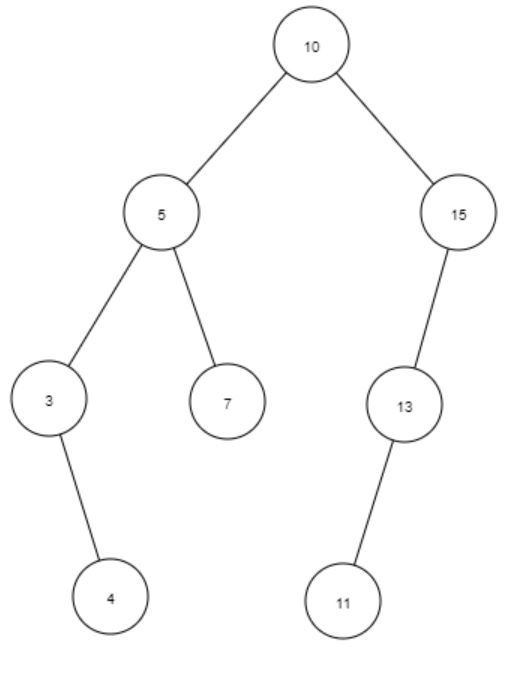
\includegraphics[width=250px, height=250px]{/trees/BST}
    \caption{The figure shows an example of a Binary Search Tree.}    
    \label{fig:BST}
\end{figure}